\documentclass[runningheads]{llncs}

%---- Sonderzeichen-------%
\usepackage[english,ngerman]{babel}
%---- Codierung----%
\usepackage[latin1]{inputenc}	% for Unix and Windows
\usepackage[T1]{fontenc}
\usepackage{graphicx}
\usepackage{url}
\usepackage{llncsdoc}
%----- Mathematischer Zeichenvorrat---%
\usepackage{amsmath}
\usepackage{amssymb}
\usepackage{enumerate}
% fuer die aktuelle Zeit
\usepackage{scrtime}
\usepackage{listings}
\usepackage{subfigure}
\usepackage{hyperref}
% multirow for specific table contents and formatting
\usepackage{multirow}
%Listings umgebung fuer dargestellte Codefragmente
\usepackage{listings}
%caption package for table captions without table environment
\usepackage{caption}
\renewcommand{\lstlistingname}{Code}

\setcounter{tocdepth}{3}
\setcounter{secnumdepth}{3}
\makeatletter
\let\@fnsymbol\@arabic
\makeatother

\mainmatter
\title{Calculating Key Performance Indicators of State Commercial Banks using Linked Open Data}
\titlerunning{Calculating KPIs using Linked Open Data}
\author{Alexander B\"uscher\thanks{alexander.buescher@inwi.org} and Andreas Harth\thanks{harth@kit.edu}}
\institute{Institute of Applied Informatics and Formal Descriptions Methods\\Karlsruhe Institute of Technology, 76131 Karlsruhe, Germany}

\authorrunning{Calculating KPIs using Linked Open Data}
\date{23.07.2007}

\begin{document}
\maketitle

\selectlanguage{english}
\begin{abstract}This research discusses possibilites and performance of Financial Data Integration on the Semantic Web context. We set up our main hypothesis: In addition to considering the bounds to our approach we took performance as well as the possible benefits to analysts work into account. By evaluating the past work regarding Semantic Web financial data representation and also combining these efforts with the benefits of a light version of the Data Envelopment Analysis we integrated data from different sources, paving the way for statistical analyses on financial data and Key Performance Indicators (KPIs). Taken together, the results of our studies show a general acceptance of all three subtopics: the disclosed use case of national banks verifies the general adaptability, the SPARQL--queries perform on a more than acceptable level and concluding overall benefits were seen by survey participants.
\end{abstract}

\section{Introduction}

The relevance of financial data is significant in the present time in several contexts. Many countries force their companies to publish quarterly and annual reports by law to ensure a maximum level of transparency. Analysts hired to detect weak points in everyday processes or improve the companies efficiency in regards of handling financial aspects are in need of a huge amount of information from different sources to handle their tasks. The presented use case is set against the background of state commercial banks listed within the United States Securities and Exchange Commission (SEC) and gives a high--level overview on possible advantages of using a Linked Data abstraction to access and integrate numerical data expressed in the Data Cube vocabulary, and out areas that require further work.\\
We aimed to present a decently performing approach in terms of generating KPIs that two (or more) data origins to be calculated.\\
Illustrating the use case by choosing state commercial banks fits our context pretty welll. The SEC lists a huge amount of companies in the commerial state bank sector, offering a reasonable quantity of information that can be contemplated within the use case. We use both in our use case to underline the relevance of data from various information systems for everyday work of analysists. Additionally the results of the evaluation support the thesis by O'Riain et al. from 2012 \cite{OCH12}, who stated that a further awareness of general facts regarding the company can lead to a competitive advantage. For exemplary illustration we included data from the SEC\footnote{\url{https://www.sec.gov/}} holding US filings and their corresponding financial reports (based on XBRL data). We also made use of the SEC data as well as Yahoo! Finance\footnote{\url{https://finance.yahoo.com}} data being dumped and formatted into Data Cube vocabulary\footnote{\url{http://w3.org/TR/vocab-data-cube/}},whereas DBpedia\footnote{\url{http://dbpedia.org/}} does not support Data Cube yet and thus does not provide information from different timestamps. Data Cube also supports our efforts to provide data for different statistical analyses in finance contexts for future work. Additionally we decided to make use of Yahoo! Finance data to be able to link developments of Key Performance Indicators (KPIs) to changes in stock prices. The general idea of the approach is graphically presented by figure 1. \\
When developing our hypothesis we suspected that the necessity of knowledge in both topics, informatics and economics, to exploit all possibilites of this approach effectively may be discouraging to some extent. After finding a suitable use case we started to work on both simple and complex queries to fullfill our requirements.\\
We address the following research questions:
\begin{enumerate}
\item are SPARQL--queries over financial data from different sources accomplishable within reasonable bounds? We tested the general practicability within reasonable bounds through a detailed discussion given by both author's evaluating possibilites, as well as advantages and disadvantages the approach discloses.
\item are they executable with good performance? we intended to point out differences in performance measuring by evaluating queries of different complexity--levels. 
\item do they ease financial analysts everday work by driving value for their customers? The driven value for both customers and analysts was proved by evaluating the results of our developed questionnaire. Thus in general it can be said that we tested whether the ascertained outputs really are relevant and helpful.
\end{enumerate}
We can now summarize the main components of our approach: By collecting and querying the (numerical) data we found available in the Data Cube format we analyse selected KPIs while making use of the DEAs characteristics and specifics.\\
Maximizing the benefits and advantages our approach could lead to was probably the biggest challenge we faced. Therefore we needed to ensure an appropriate knowledge of both economics and informatics. By this point we focussed on queries handling with important numbers to customer and analysts. Our work provides highly configurable queries that can be adopted to other scenarios and branches. Furthermore we offer reproducible outputs by providing queries and practices as well as instructions via GitHub\footnote{\url{https://github.com/abuescher/financial-linked-open-data-integration}}. Thereby generated data can be used for statistical analyses in finance contexts. We also present possibilites offered when using
\begin{figure}[!t]
\centering
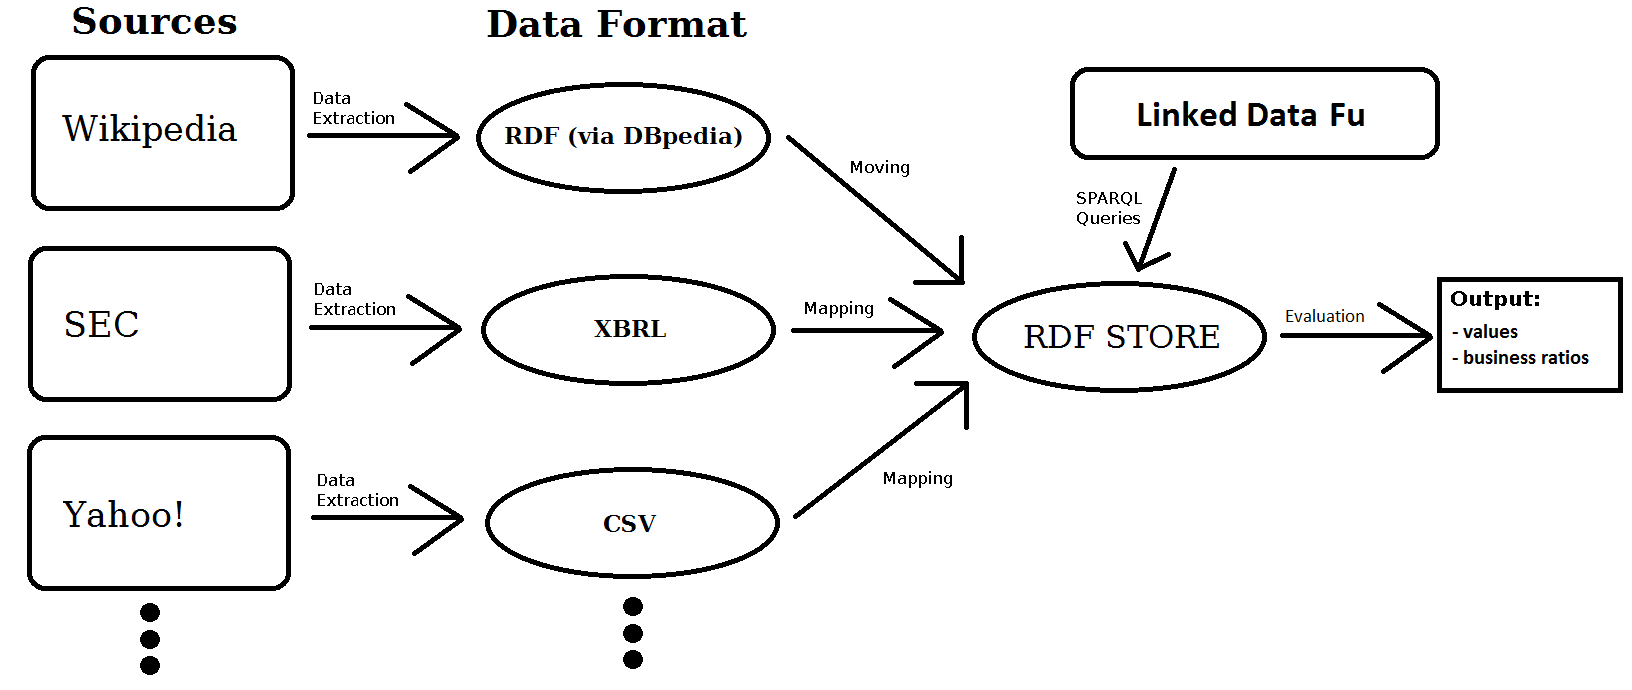
\includegraphics[scale=0.2]{1_graphics/extract_neu.png}
\caption{Data integration from various sources -- adopted from \cite{KWOW14}}
\end{figure}
Linked Data Fu tool to interested parties \cite{SSHS13}. When executed correctly our approach can simplify (statistical) competitors analysis including arbitrary choice of KPIs an analyst may want to compare, provided the needed data is available.
\section{Conceptional background and related work}
\label{c2}
The presented process of hypothesis development requires some previous information to be understood properly. Especially knowledge in the current research state regarding translations from eXtensible Business Reporting Language (XBRL), which is used to present financial statements via eXtensible Markup Language (XML) syntax, to Resource Description Framework (RDF), basics of the Data Envelopment Analysis (DEA) and the Linked Data Fu, which was used to test both general usability and performance of the queries, is needed.\\
First of all the the necessarity was given to be able to convert data from the XBRL format into RDF to ensure further possibilites and more flexibility in regards of data analysis \cite{Mill98} from different sources. Our approach evualuates three different procedures before coming to the conclusion that the one from K\"ampgen et al. \cite{KWOW14} fits the given context and the hypothesis that is to be proven best. The reasons behind dropping the two other approaches out of consideration were that XBRL instance documents and their corresponding taxonomies were translated seperated from each other and into different languages (\cite{GaGi10}, \cite{BRLD10}).\\
Furthermore, basic knowledge of the economical topic of Data Envelopment Analysis (DEA) is needed. The light--weighted version makes use of the simple rule that every output a company generates can be divided through any input that influences the company and its products or service, as long as both are quantifiable and non--negative values (\cite{Schu14}, \cite{Wei01}). We use these facts to compute relevant business ratios in the use cases context \cite{CeCP08} with inputs and outputs integrated from different data origins.\\
At this point all preperations needed to fill up our RDF store with data from different sources are made. To enable data analysis and performance tests, we needed software to run SPARQL--queries above these store, as shown in Fig. 1. Thus we used the Linked Data Fu \cite{SSHS13}. This tool makes it possible to run queries of different level of complexity on local systems. Given a datastore the programs output is the specific amount of triples that meet all requirements of the given query. Chapter \ref{6.2.} presents the results of these tests.
\section{Use Case}
The following chapter presents the selected use case for our approach. We don't intend to go on reasons for selecting this specific sector in detail. Please note that there were some sector restricted measures that can be adapted to other sectors. Further measures can be applied to all different kinds of sectors.
\subsection{Preperations}
While all knowledge and content related requirements have been met now, there is a small technical addition needs to be provided as well, before presenting the case. The arguably most important aspect of this approach includes the possibility of data integration from various sources. The initial datastore only consists of triples linking two sources\footnote{Please find paths to the used prefixes on \url{http://prefix.cc/}.}
\begin{lstlisting}[caption= Linking resources using the owl:sameAs property]
edgarcik:{CIK#id} owl:sameAs dbpedia:corresponding_bank .
\end{lstlisting}
This example shows the general idea how we linked different sources. Please note that the CIK number (\{CIK\#id\} in this illustration) needs to be replaced with the actual CIK number of the considered bank. \\
Also bear in mind that this example shows the connection between the SEC and DBpedia data. More data sources can be easily integrated by replacing the DBpedia URI with the source to be integrated (e.g. Yahoo!Finance). Therefore the needed triple has to be added for every bank and every source exactly \textbf{once}. \\
Having these links set up, we enhanced our queries by an additional part\footnotemark[6]:
\begin{lstlisting}[caption= Using httpm:GET to access data from different sources]
{
  ?companySEC edgar:cikNumber ?number .
  ?companySEC owl:sameAs ?companyNewSource .
} = > {
[] http:mthd httpm:GET ;
   http:requestURI ?companyNewSource . } .
\end{lstlisting}
We appropriate the HTTP GET method to ensure that we can use information from the integrated data source. In the given example we would be able to include data from all origins that were linked with the triple presented in Code 1.1. The next chapter shows the usability in different scenarios.
\subsection{Key Performance Indicators (KPIs) selection}
\label{3.2}
The selection of key figures is a difficult, complex and non--structured task. In our context of bank performance multiple different approaches have been made \cite{KPDZ06} -- a significant proportion came to the conclusion that only taking standardised figures into consideration, will not necessarily lead to reliable statements regarding performance (e.g. \cite{HaSC97} and \cite{BhSh07}). \\
After taking a large amount of different data into consideration, we downsized them to a total number of five KPIs to be evaluated in our use case.
\subsubsection{Total turnover per employee:}
First, we took the total turnover per employee \cite{SeZh99} into our interpretations:
\begin{equation}
\frac{totalTurnover}{numberOfEmployees}
\end{equation}
This is the first time we make use of our link between the representing URIs of the SEC data as well as the corresponding DBpedia index.
\subsubsection{Production efficiency:}
A very interesting point in the context of state commercial banks is their evaluation in terms of production effectiveness, as banks do not have a production in the classical sense. Giokas \cite{Gio08} splitted the efficiency as a whole into three seperated and independent parts: "Production Efficiency", "Transcation Efficiency" and "Intermediation Efficiency". We decided to choose the Production effeciency to be evaluated more detailed.\\
Wu concluded that the production effectiveness of banks can be evaluated by dividing the Non--interest income through the accumulated personnel costs (Table 1,\cite{Wu12}):
\begin{equation}
\frac{Non-interestIncome}{PersonnelCosts}
\end{equation}
Both needed information can be extracted from the appropriative SEC documents.
\subsubsection{Total turnover per location:}
Another important aspect in context of choosing a bank institution is the geographical penetration \cite{DeGe05}. We determine this KPI by dividing the total turnover through the number of offices a company has:
\begin{equation}
\frac{totalTurnover}{numberOfLocations}
\end{equation}
To compute this KPI, we repeatedly made use of the DEA's characteristics and also integrated data from two different sources, namely the SEC and DBpedia.
\subsubsection{Gains and losses for multiple periods:}
One of the most basic KPIs are gains and losses companies observed. Long--term losses and gains are one of the most significant parameters when it comes to judging reliability and stability of banks \cite{AlGa09}:
\begin{equation}
\sum_{t=0}^{n}NetIncomeLoss(t)
\end{equation}
There is another reason for taking losses and gains into our consideration. We suspect these to demonstrate the most significant impact on the chart--development in regards of the price of a companies shares, which will be tested within the next and final part of the use case that shows a preview on the possibility to test different impacts on the price of shares.
\subsubsection{Prospect -- Price of shares:}
Considering the integration from share--related data, we could analyse the effect of different key figures on their price development. By comparing the trends of both the considered characteristic number as well as the price of shares, we could give answers on two impotant questions:
\begin{enumerate}
\item Does the considered characteristic impact the price of shares at all?
\item If present, how large is the impact?
\end{enumerate}
Table 1 sums up all chosen KPIs as well as their corresponding URIs presenting the needed data from different sources. \\ \\
Below we present some exemplary outputs from the given KPIs. We used an examplary company to make our approach more concrete. Please note that the presented examples can be adapted to any other listed SEC filing easily -- this also applies to data from Yahoo or DBpedia. For our illustrations we used the given information of the Fifth Third Bancorp\footnote{\url{https://www.53.com/site}} from various sources\footnote{\url{http://www.sec.gov/cgi-bin/browse-edgar?action=getcompany&CIK=35527}} \footnote{\url{http://dbpedia.org/resource/Fifth_Third_Bank}} \footnote{\url{http://finance.yahoo.com/q?s=FITB}} as well as available information of Wilmington Trust Corp\footnote{\url{https://www.wilmingtontrust.com/}}.
\begin{table}[!h]
\begin{tabular}{|c|c|c|c|}
\hline
\textbf{No.} & \textbf{KPI} & \textbf{Data origin(s)} & \textbf{Corresponding URIs} \\
\hline
\hline
\multirow{2}{*}{1} & \multirow{2}{*}{ $\frac{totalTurnover}{numberOfLocations}$} & SEC & us-gaap2009:totalTurnover\\
 & & DBpedia & dbpedia-owl:numberOfEmployees\\
\hline
\multirow{2}{*}{2} & \multirow{2}{*}{ $\frac{Non-interestIncome}{PersonnelCosts}$ } & SEC & us-gaap2009:noninterestIncome\\
 & & SEC & us-gaap2009:LaborAndRelatedExpense\\
\hline
\multirow{2}{*}{3} & \multirow{2}{*}{ $\frac{totalTurnover}{numberOfLocations}$} & SEC & us-gaap2009:totalTurnover\\
 & & DBpedia & dbpedia-owl:numberOfLocations\\
\hline
4 & $\sum_{t=0}^{n}NetIncomeLoss(t)$ & SEC & us-gaap2009:NetIncomeLoss \\ 
\hline
\multirow{2}{*}{5} & \multirow{2}{*}{Price of shares} & SEC & -- \\
 & & Yahoo &yahoo:Close\\
\hline
\end{tabular}
\label{table1}
\caption{Overview of the considered KPIs in the presented case}
\end{table}
\subsection{Results}
For our result section we divided our tests into two parts:
\begin{enumerate}
\item individual performance tests regarding the previously listed KPIs
\item a competitors analysis, showing results from different companies on particular key figures
\end{enumerate}
Table 2 illustrates the Fifth Third Bancorp's development over one year in terms of production efficiency while table 3 gives an example of an output of the competitors analysis considering the total turnover per employee as chosen KPI. \\
The upcoming chapter presents our evaluation's methodology. 

\section{Methodology}
The simplification of financial analysts everyday work and driving value to the customer is one of the three parts of our main hypothesis. In order to test this aspect we decided to conduct a survey and present our findings to an appropriate audience.
\subsection{Design and sample}
To be able to recognize the whole possibilities our approach presents, we needed participants who exhibit a basic knowledge in both informatics (Semantic Web in the best case) and economics. Therefore we had chosen our sample to be all students of Information Engineering and Management who exactly offer the needed expertise for our case \cite{GeTa03}. \\
The questionnaire was inspired by the work of Weijters et al. from 2010 \cite{WeCS10} and Weathers et al. from 2005 \cite{WeSN05}. Both drew the conclusion that five point likert scales (fully labeled) lead to the best results in terms of validity
\begin{table}
\centering
\begin{tabular}[htp]{|c|c|c|}
\hline
\textbf{?result} & \textbf{?nonInterestIncome} &  \textbf{?personnelCosts}\\
\hline
\hline
1.262 & 3267000000 & 2874000000\\
\hline
1.338 & 3967000000 & 2965000000\\
\hline
\end{tabular}
\caption{Fifth Third Bancorp production efficiency 2009 and 2010}
\end{table}
\begin{table}
\centering
\begin{tabular}[htp]{|c|c|c|}
\hline
\textbf{?result} & \textbf{?cikNr} & \textbf{?name} \\
\hline
\hline
431915 & 35527 & FIFTH THIRD BANCORP\\
\hline
332087 & 22356 & COMMERCE BANKSHARES INC\\
\hline
322478 & 36270 & M\&T BANK CORP\\
\hline
\end{tabular}
\caption{Competitors analysis -- turnover per employees (excerpt)}
\end{table}
and response bias. The questionnaire consisted of two parts. In the first part all participants were asked to estimate their knowledge in terms of informatics and economics in general and in terms of Semantic Web and Finance and Accounting specifically.
The second part of the survey consists of nine statements. All participants were asked to rank their degree of acceptance respectively refusal on a five--point likert scala. The scala had all five positions labeled: "Stimme zu" (strongly agree), "Stimme eher zu" (slightly agree), "Neutral" (neutral), "Stimme eher nicht zu" (slightly disagree) and "Stimme nicht zu" (strongly disagree). \\
We randomly chose a total number of 15 students as participants for our survey, representing 2.85\%\footnote{status as of October, 2014} of all Information Engineering and Management student's of the Karlsruhe Institute of Technology (KIT). In groups of three people a short and objective lecture was hold that pointed out the basic ideas of the approach. Afterwards the survey was handed out to attendees.
\subsection{Quality measurements}
When designing the questionnaire we took quality management into our considerations. Inspired by the work of Weathers et al. from 2008 \cite{SwWN08} we decided to include three reversed--item pairs into the survey to ensure an appropriate grade of validity and consistency. \\
In the next step we defined a misresponse to a reversed--item pair. By doing so we determined that in our case a misresponse is rating the first half of the pair with "strongly agree" or "slightly agree" while \textbf{not} rating the second part of the pair with either "strongly disagree" or "slightly disagree" and vice versa. Rating one part of the reversed--item pair with "neutral" leaves the pair without misresponse. These calculations leave us with three potential misresponses per participant and thus a maximum of 45 in total. Only \textbf{one} of these possible 45 mistakes has been done resulting in the satisfying number of only about 2.22\% misresponse to reversed--items. \\
Additionally we decided to evaluate our internal consistency by computing the standardised Cronbach's alpha \cite{TaDe11}. We took advantage of the specific rule for likert scales: $\alpha_{st} \le \alpha_u$ with $\alpha_{st}$ being the standardised Cronbach's alpha and $\alpha_u$ being the usual one. After computing $\alpha_{st} = 0.7441$ we could already state our internal consistency as acceptable \cite{Geor03}. \\
\section{Evaluation and findings}
In terms of structuring the evaluation we stuck to our threefolded hypothesis. In the first part a detailed analysis, discussing advantages as well as disadvantages from our point of view is given. The second subtopic consists of hard facts as results of our performance tests. The chapter closes with a reporting on given opinions from our survey's participants and the conclusions we drew.
\subsection{Discussion}
We faced the task of an appropriate choice of KPIs. In this context we do not only speak of the right amount of different examples but also of figures we can access the needed information for. As trivial this may sound, the challenge turned out tremendous. However, we were able to determine significant and exemplarily adequate figures so we could point out a total amount of five examples that illustrate possibilities and restrictions quite well. \\
In terms of complexity we met mixed experiences. The DEA itself was easily adapted and fitted the context of data integration from various sources acceptably well. Escpecially in terms of the competitors analysis we had to deal with bigger and more complicated SPARQL--queries. Therefore we evaluated queries above a way larger datastore than for other queries, which obviously leaded to inferior performance results, as will be presented in the next chapter. \\
A promising prospect is given by the use of the fifth key figure (integration from Yahoo stock data linked to data from the SEC). The approach knows how to demonstrate his advantages and opportunities especially when it comes to dynamic interactions between different numbers. Analysts can easily determine if there is an impact from one KPI on another.\\
One negative aspect is the connection between two data origins that has to be inserted by hand once (cf. code 1.1), which takes about 30 seconds up to one minute for every inserted bank. A possible workaround is an automatically handling of newly inserted companies into the initial datastore. Once a company is added to the datastore for the first time the link between the SEC dump and the corresponding sources is generated automatically by making use of their connected name linked via the foaf:name property. Obviously there can be differences between this attribute and the URI representing the corresponding company that have to be dealt with.\\
Concluding we can record the general confirmation of the first subtopic of the main hypothesis. First of all there are bounds to our approach without any doubt. The most problematic aspect is probably the difference in publications in XBRL, meaning the possibilites for companies to introduce their own financial facts by defining them in their own taxonomy documents. Replacing the usually used financial facts with these specially developed ones significantly impairs to ensure the general usability. Besides that there is no question that the demanded accomplishments could be presented by our use case and thus generally support the first part of our main hypothesis.
\subsection{Performance}
\label{6.2.}
For our performance tests we ran the different queries on our server: 2x Intel(R) Xeon(R) CPU E5-2670 0 @ 2.60GHz CPU, consisting of 128 GB memory (RAM) and running on 16 cores (32 with Hyperthreading). To ensure that our tests delivered both comparable and qualitative results we started all tests when the CPU load showed (nearly) 0\%.
\begin{table}
\centering
\begin{tabular}{|c|c|c|c|c|}
\hline
\textbf{No.} & \textbf{Data origin(s)} & \textbf{Incl. http:GET} & \textbf{Excl. http:GET} & \textbf{\# of triples}\\
\hline
\hline
1 & SEC + DBpedia & 15m32s & 3.16s & 55.000\\
\hline
2 & SEC & 13m58s & 2.79s & 51.000\\
\hline
3 & SEC + DBpedia & 15m42s & 3.55s & 55.000\\
\hline
4 & SEC & 13m48s & 2.88s & 51.000\\
\hline
5 & SEC + Yahoo & 17m02s & 11.30s & 1.203.000\\
\hline
All & SEC + DBpedia + Yahoo & 18m14s & 25.24s & 1.211.000\\
\hline
\end{tabular}
\caption{Performance test results}
\end{table}
All tests were performed with version 0.9.3 of the Linked Data Fu \cite{SSHS13}. While the first five queries accord to the listing in table 1 the sixth call evaluated all five previous queries and  their corresponding output in one single call.\footnote{Please find more examples for querying Linked Open financial data on GitHub: \url{https://github.com/abuescher/financial-linked-open-data-integration}} We divided our tests into two different procedures. The first approach integrated data and evaluated queries live, which means evaluated data was included in real--time by using http:get on considered sources. The second one evaluated queries over an already built dataset, which can be updated on a regular base.\\
One aspect that extends the needed execution time slightly is including data from DBpedia and especially Yahoo compared to only using information from the SEC documents. The times indicate the commensurability of the trade--off between complexity and performance. Concluding the practicability with good performance can still be seen as supported.
\subsection{Survey results}
Our survey aimed on two different aspects. On the one hand we wanted to evaluate how much prior knowledge in topics of both Semantic Web and finance and accounting are needed to feel comfortable with our approach. On the other hand it was our intention to point out the significance of our illustrations for companies. According to our needs we designed 13 questions.\\
The evaluation fits our hypothesis well. We asked the participants to give us their impressions on the usability and relevance from a companies point of view. Additionally we requested them to estimate whether companies would use our approach or not. About 73\% stated that they support the statement, saying companies would use the concept. Also about 93\% respectively 98\% supported our perception on usability and relevance.\\
The results from our evaluation on needed prior knowledge turn out similarly positive. While about 40\% of the participants estimated their prior knowledge in informatics above average, only 26\% did so in the Semantic Web context. Still approx. 75\% supported our presentation of an easy to adapt approach. Even though survey attendees ranked their knowledge in terms of general topics in business economics (approx. 80\% above average) and in finance and accounting in particular (approx. 53\% above average) quite high, we still sicern our thesis supported in terms of a low degree of complexity. \\
As already mentioned before we secured data validity and quality by two concepts (reversed--item pairs and Cronbach's alpha) which both approve our methodology in these terms.\\ 
At the end of this chapter it can be said that independent quality tests underline both consistency and vailidity of the survey's design and thus our results supporting the third and final part of the main hypothesis.
\section{Conclusion}
Concluding we find all three subtopics of our main hypothesis supported in general. There can be discussions whether the bounds to our approach are reasonable or not without doubt. Yet there is no discussion regarding the decent performance as well as the general adaptability without needing a deep and detailed prior knowledge. Our approach is applicable to other sectors, companies and KPIs. In order to extend it one would need to add the owl:sameAs relationship for broader companies to the initial data store respectively develop and carry out queries that extract the needed information for further KPIs.
% Normaler LNCS Zitierstil
%\bibliographystyle{splncs}
\bibliographystyle{itmalpha}
\bibliography{literatur}
\end{document}

